% These are full figures for the appendix

\begin{figure*}
  \centering
  \newcommand{\gsize}{.45\textwidth}
\begin{tabular}{c| c c}
    \hline\hline
  & \textbf{OT-Based (GMW)} & \textbf{Beaver Triple-Based}\\
    \hline\hline
  \rotatebox{90}{\phantom{helloh}$i = 128, n = 1024$}
  & 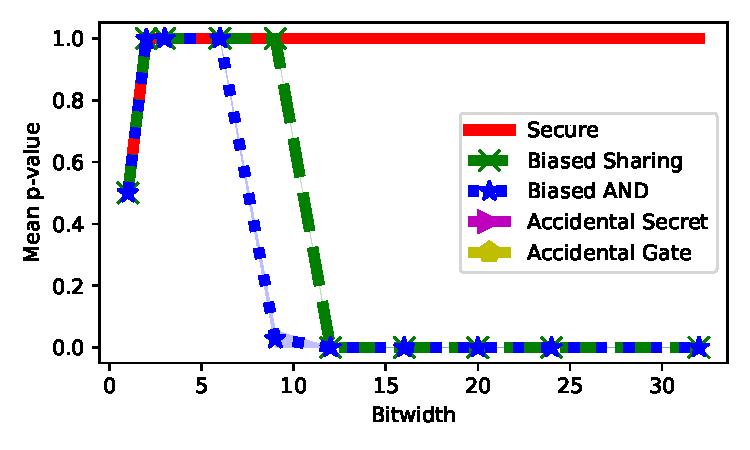
\includegraphics[width=\gsize]{graphs/security_adder_gmw_128_1024.pdf}
                 & 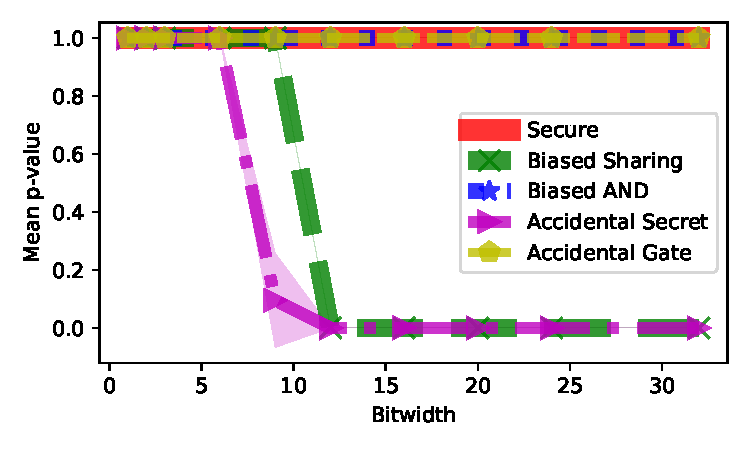
\includegraphics[width=\gsize]{graphs/security_adder_beaver_128_1024.pdf} \\
    \hline
  \rotatebox{90}{\phantom{helloh}$i = 128, n = 2048$}
  & 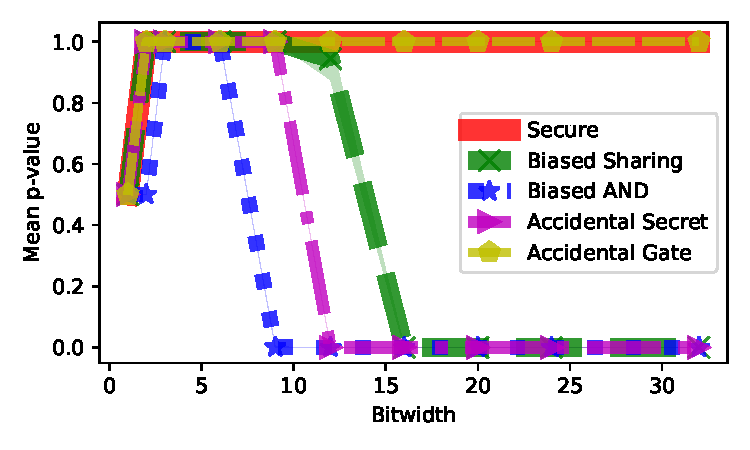
\includegraphics[width=\gsize]{graphs/security_adder_gmw_128_2048.pdf}
                 & 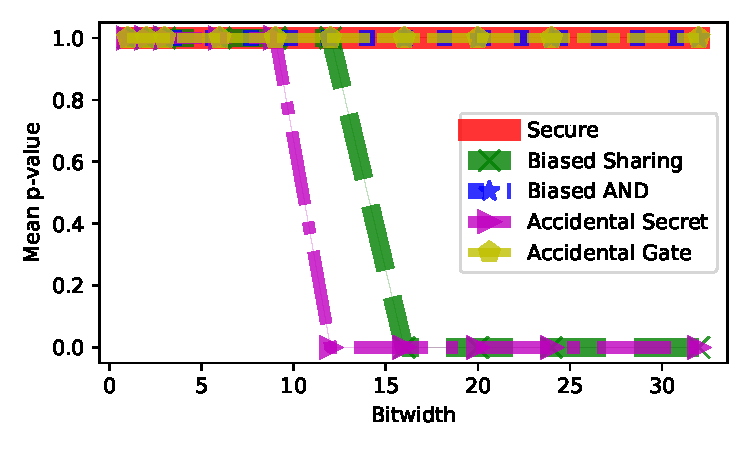
\includegraphics[width=\gsize]{graphs/security_adder_beaver_128_2048.pdf} \\
    \hline
  \rotatebox{90}{\phantom{helloh}$i = 256, n = 1024$}
  & 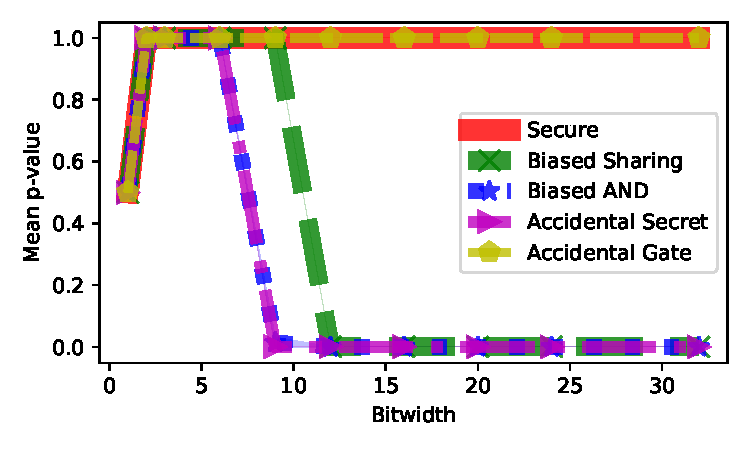
\includegraphics[width=\gsize]{graphs/security_adder_gmw_256_1024.pdf}
                 & 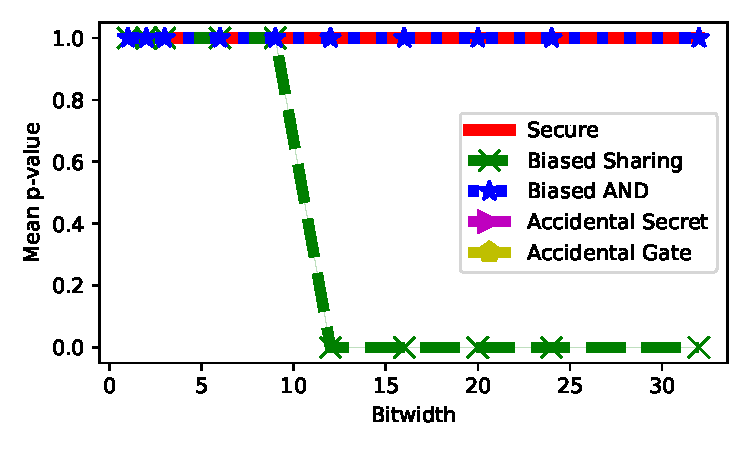
\includegraphics[width=\gsize]{graphs/security_adder_beaver_256_1024.pdf} \\
    \hline
  \rotatebox{90}{\phantom{helloh}$i = 256, n = 2048$}
  & 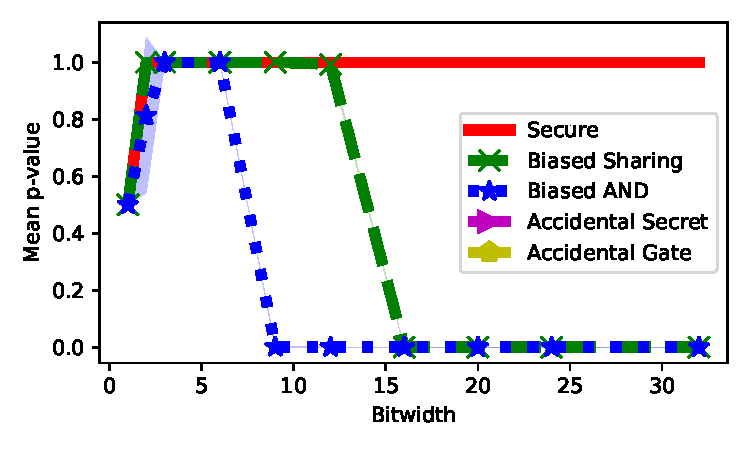
\includegraphics[width=\gsize]{graphs/security_adder_gmw_256_2048.pdf}
                 & 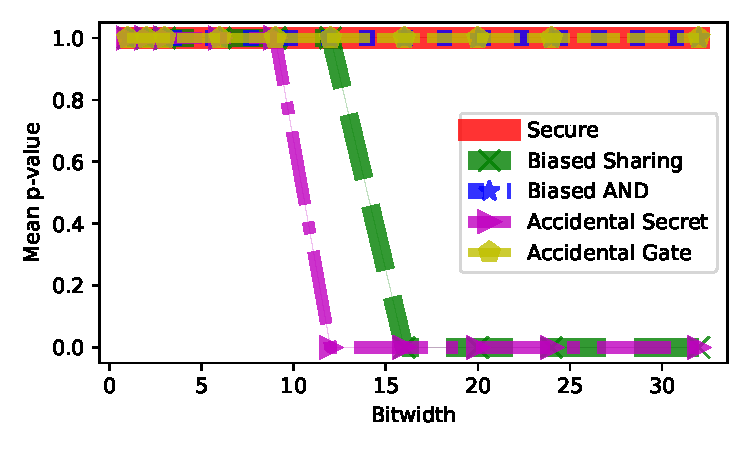
\includegraphics[width=\gsize]{graphs/security_adder_beaver_256_2048.pdf} \\
    \hline
    \hline
\end{tabular}
\caption{Experimental results, $n$-bit addition.}
\label{fig:extra1}
\end{figure*}

\begin{figure*}
  \centering
  \newcommand{\gsize}{.45\textwidth}
\begin{tabular}{c| c c}
    \hline\hline
  & \textbf{OT-Based (GMW)} & \textbf{Beaver Triple-Based}\\
    \hline\hline
  \rotatebox{90}{\phantom{helloh}$i = 128, n = 1024$}
  & 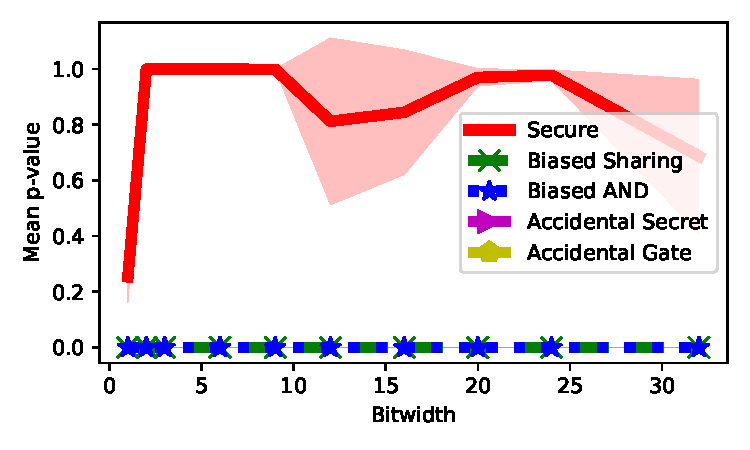
\includegraphics[width=\gsize]{graphs/security_less_than_gmw_128_1024.pdf}
                 & 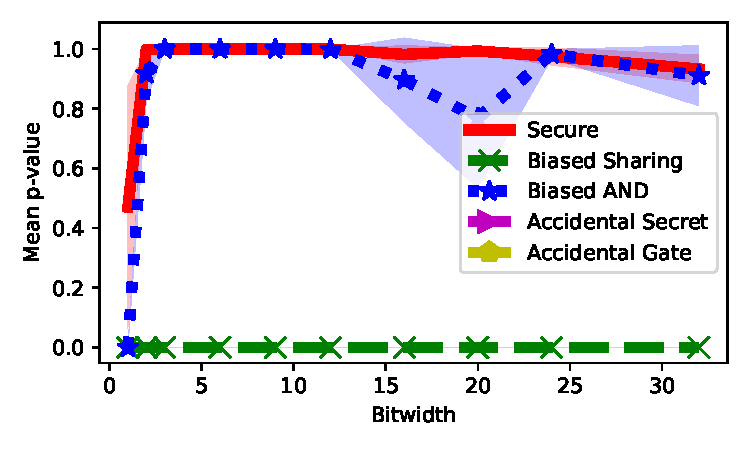
\includegraphics[width=\gsize]{graphs/security_less_than_beaver_128_1024.pdf} \\
    \hline
  \rotatebox{90}{\phantom{helloh}$i = 128, n = 2048$}
  & 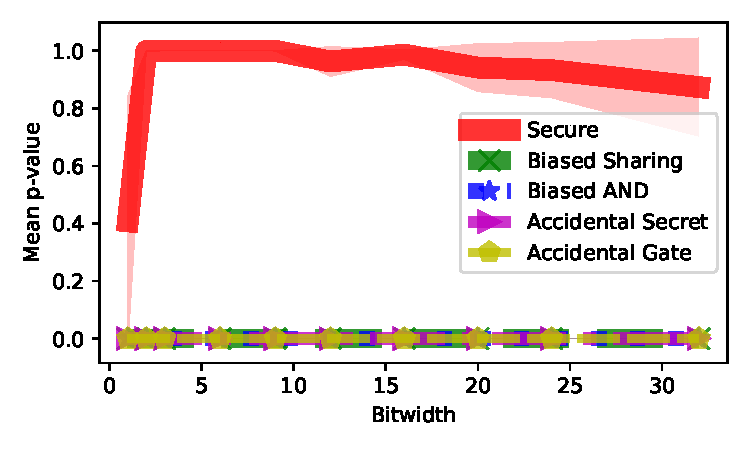
\includegraphics[width=\gsize]{graphs/security_less_than_gmw_128_2048.pdf}
                 & 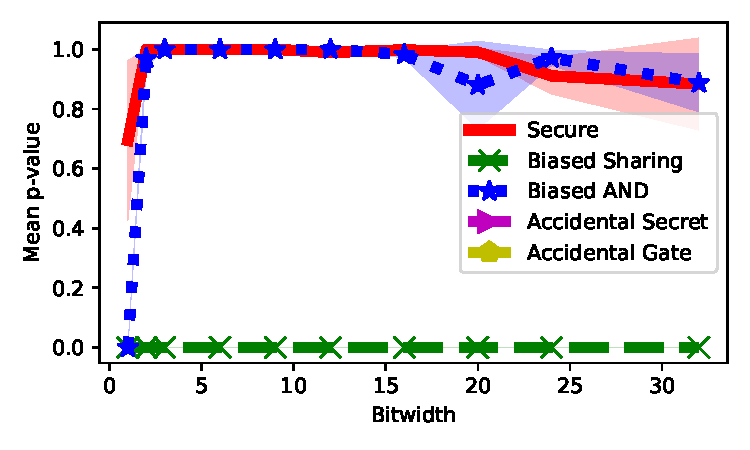
\includegraphics[width=\gsize]{graphs/security_less_than_beaver_128_2048.pdf} \\
    \hline
  \rotatebox{90}{\phantom{helloh}$i = 256, n = 1024$}
  & 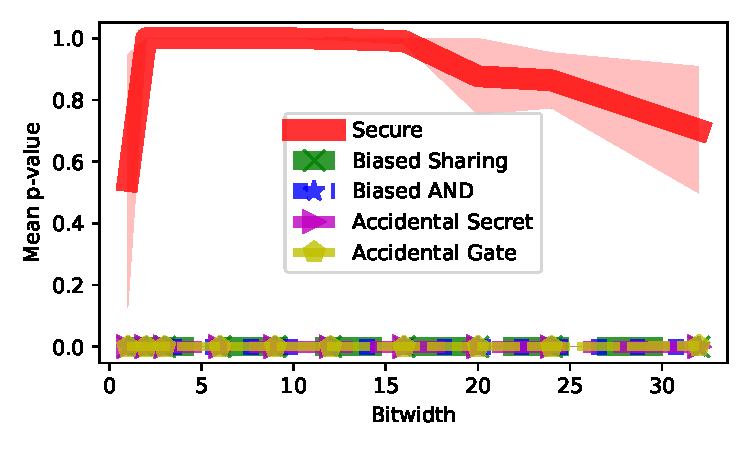
\includegraphics[width=\gsize]{graphs/security_less_than_gmw_256_1024.pdf}
                 & 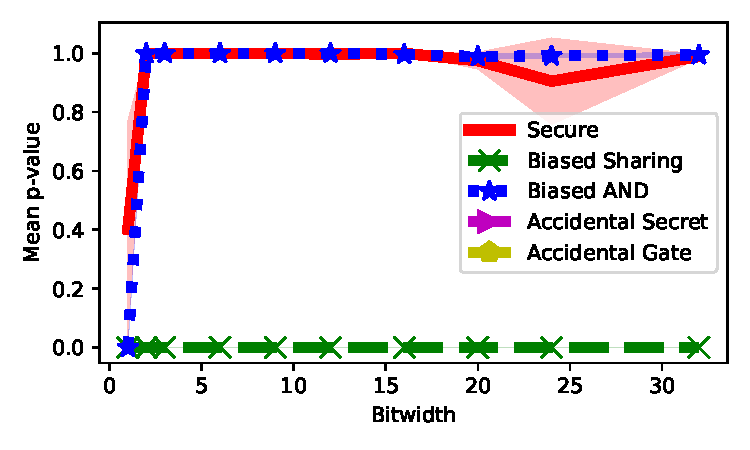
\includegraphics[width=\gsize]{graphs/security_less_than_beaver_256_1024.pdf} \\
    \hline
  \rotatebox{90}{\phantom{helloh}$i = 256, n = 2048$}
  & 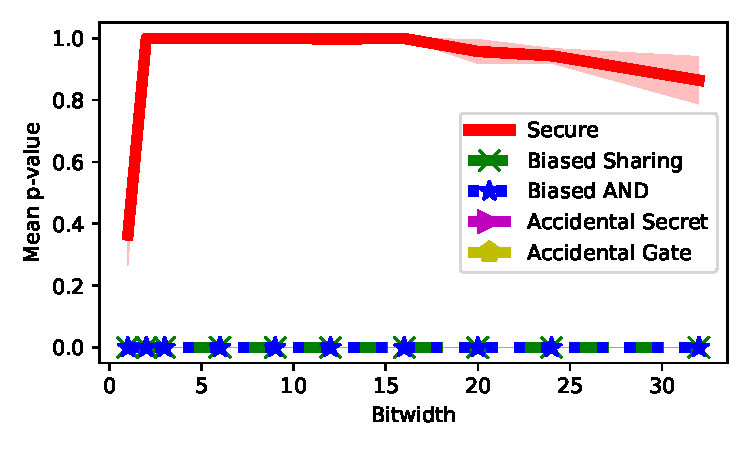
\includegraphics[width=\gsize]{graphs/security_less_than_gmw_256_2048.pdf}
                 & 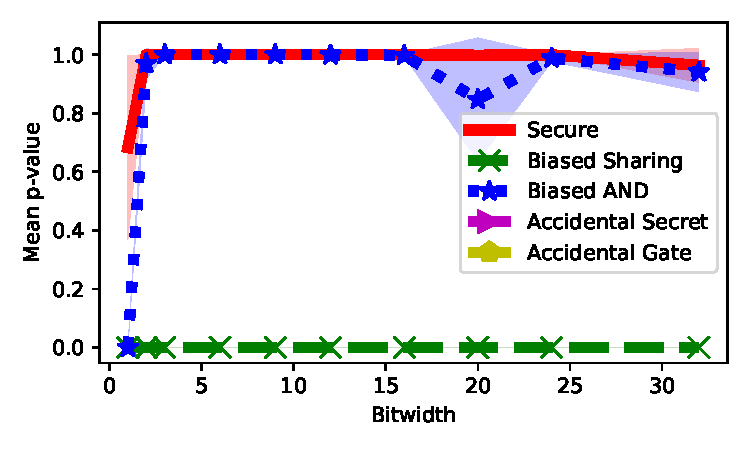
\includegraphics[width=\gsize]{graphs/security_less_than_beaver_256_2048.pdf} \\
    \hline
    \hline
\end{tabular}
\caption{Experimental results, $n$-bit less-than comparison.}
\label{fig:extra2}
\end{figure*}

\begin{figure*}
  \centering
  \newcommand{\gsize}{.45\textwidth}
\begin{tabular}{c| c c}
    \hline\hline
  & \textbf{OT-Based (GMW)} & \textbf{Beaver Triple-Based}\\
    \hline\hline
  \rotatebox{90}{\phantom{helloh}$i = 128, n = 1024$}
  & 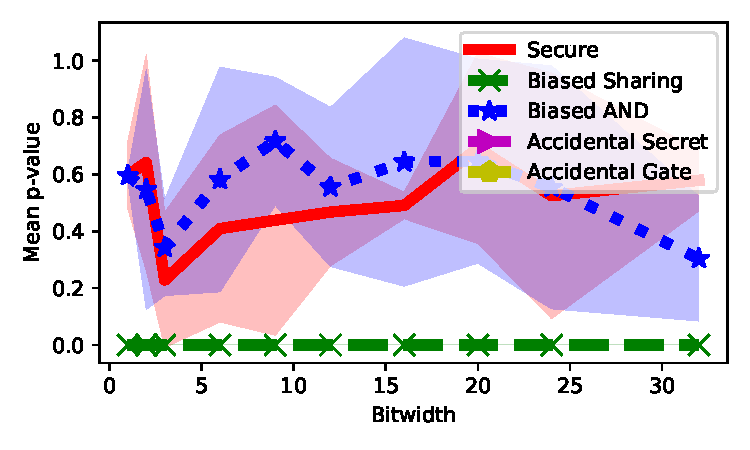
\includegraphics[width=\gsize]{graphs/security_beaver_triple_gen_gmw_128_1024.pdf}
                 & 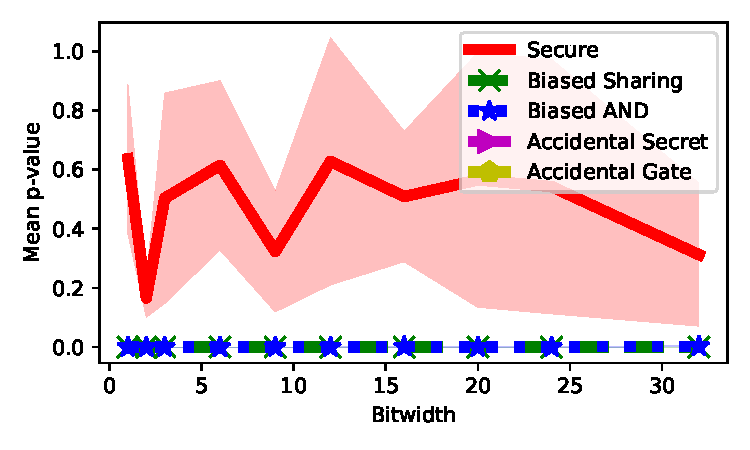
\includegraphics[width=\gsize]{graphs/security_beaver_triple_gen_beaver_128_1024.pdf} \\
    \hline
  \rotatebox{90}{\phantom{helloh}$i = 128, n = 2048$}
  & 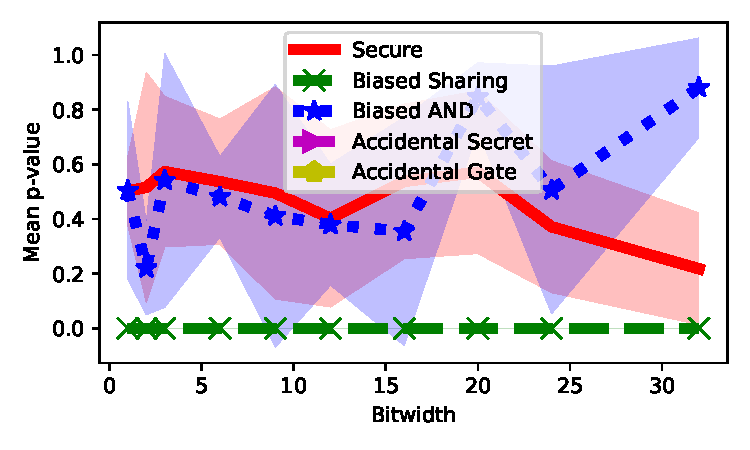
\includegraphics[width=\gsize]{graphs/security_beaver_triple_gen_gmw_128_2048.pdf}
                 & 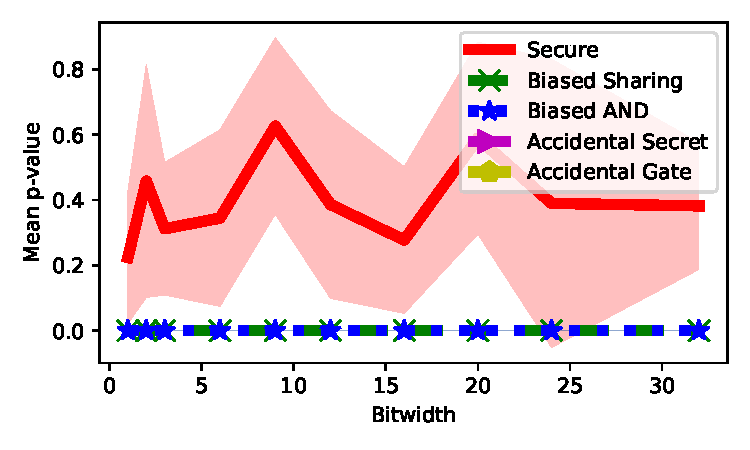
\includegraphics[width=\gsize]{graphs/security_beaver_triple_gen_beaver_128_2048.pdf} \\
    \hline
  \rotatebox{90}{\phantom{helloh}$i = 256, n = 1024$}
  & 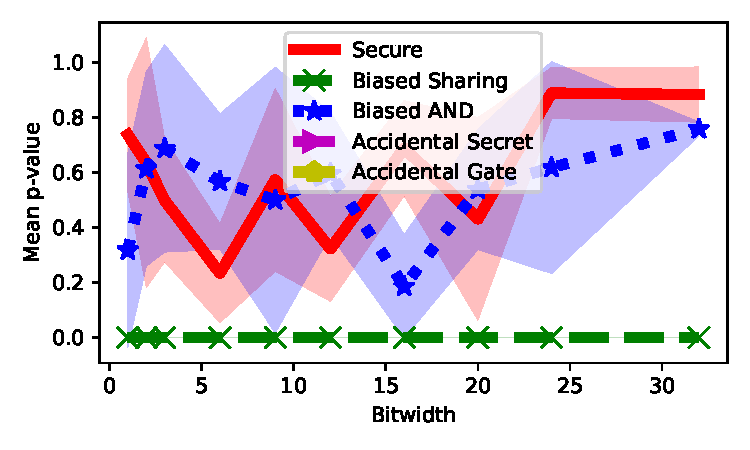
\includegraphics[width=\gsize]{graphs/security_beaver_triple_gen_gmw_256_1024.pdf}
                 & 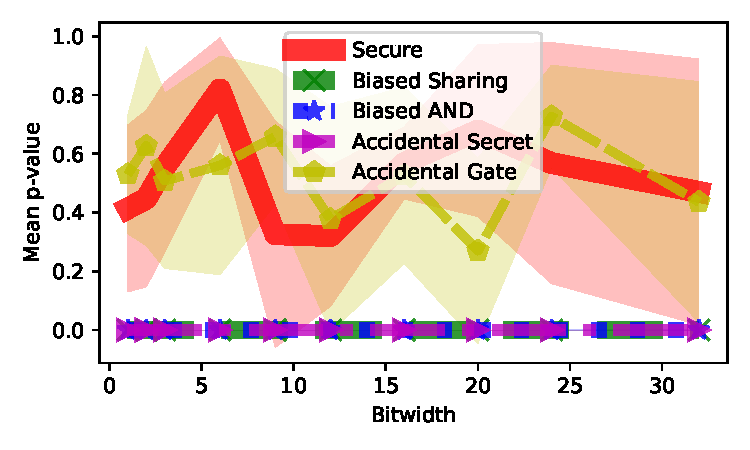
\includegraphics[width=\gsize]{graphs/security_beaver_triple_gen_beaver_256_1024.pdf} \\
    \hline
  \rotatebox{90}{\phantom{helloh}$i = 256, n = 2048$}
  & 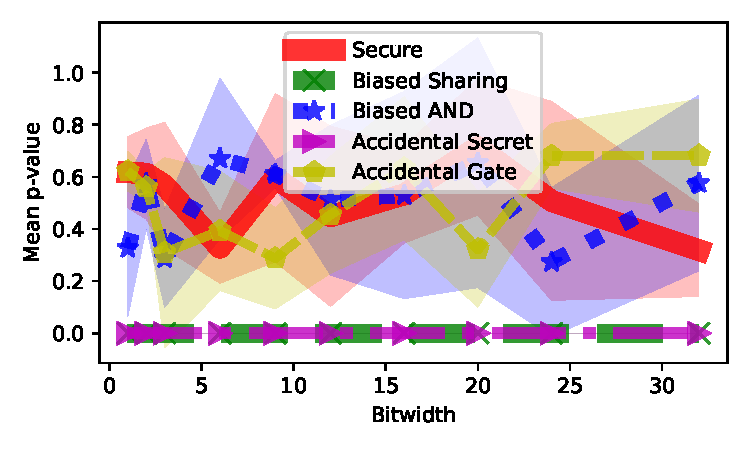
\includegraphics[width=\gsize]{graphs/security_beaver_triple_gen_gmw_256_2048.pdf}
                 & 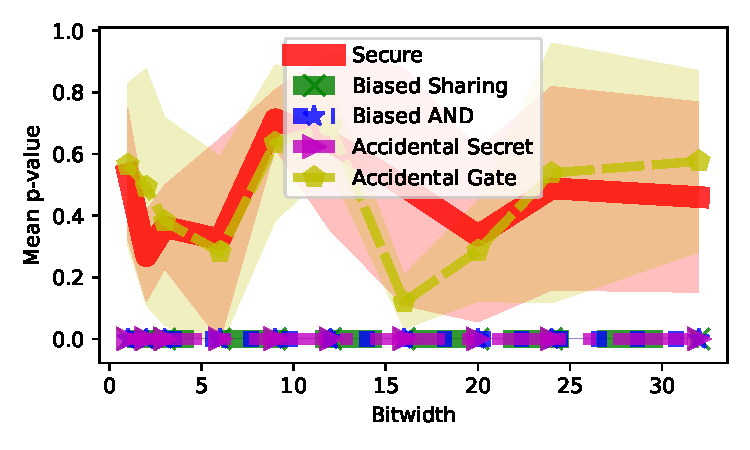
\includegraphics[width=\gsize]{graphs/security_beaver_triple_gen_beaver_256_2048.pdf} \\
    \hline
    \hline
\end{tabular}
\caption{Experimental results, $n$-bit Beaver triple generation.}
\label{fig:extra3}
\end{figure*}


